\documentclass[a4paper, 12pt]{report}

\usepackage{longtable}
\usepackage{lipsum}					    % Als Platzhalter f�r gewisse Stellen
\usepackage{ngerman}					%Deutsche Silbentrennung etc.
\usepackage[latin1]{inputenc}        	% Umlaute in .tex Files normal schreibbar
% Unter texnic-center alle Quelldateien unter Codierung ANSI abspeichern
% Auf Unixsystemen ISO 8859-15
\usepackage{helvet}						%Helvetic als Schriftart
\usepackage{courier}					%Courier als Schriftart f�r Listings
\usepackage{fancyhdr}					%Kopf- und Fu�zeilen �ndern
\usepackage{a4}								%A4 Randeinstellungen
\usepackage{makeidx}					%Indexkommandos
\usepackage{listings}					%F�r zeilennummerierte Listings mit Hintergrund
\usepackage{color}					    %F�r grauen Hintergrund in Listings
\usepackage{setspace}					%Gr��erer Zeilenabstand
\usepackage{graphicx}					%Grafiken einbinden
\usepackage{sectsty}					%Format der �berschriften um�ndern
\usepackage{hyperref}
\usepackage{float}
\usepackage{pdfpages}					%Fremde pdfs einbinden
\usepackage[font={scriptsize}]{caption}
\usepackage{verbatim} %multiline comments
\usepackage{placeins} %tableplacement
%Dokumentationen zu den Paketen finden sich im Installationsordner 
%(normalerweise C:\Programme\texmf) unter docs und dort auch im Unterverzeichnis latex.

%Das Kompilieren des Dokuments ben�tigt bis zu 3 Durchl�ufe im alle Referenzen und
%Literatureintr�ge korrekt einzubinden.

%----------------------------------------------------------------------------------
% Listings 
%----------------------------------------------------------------------------------

%Definition des Aussehens der externen Listings
\def\source#1#2#3{     %  Sprache, Caption, Dateiname 
  %\global\advance\Sourcenummer by 1 
  %\index{Listing #1 #2}
  %\textbf{Listing-\the\Sourcenummer: #2}
  \lstinputlisting[language=#1,caption=#2]{#3} 
}

% Beispiele f�r eine Verwendung
%--------------------------------------------------------------------------------
% \source{xml}{\texttt{faces-config.xml}}{sources/faces-config.xml}
%
% \source{java}{\texttt{beans.UserBean.java}}{sources/jsf/user/UserBean.java}
%---------------------------------------------------------------------------------


%Definition des Aussehens der internen Listings
\definecolor{listinggray}{gray}{1.0}

%-------------------------------------------------------------------------
% Neues Listingformat
% --- kleine Schrift
% --- Keywords f�rbig
%-------------------------------------------------------------------------

\definecolor{dkgreen}{rgb}{0,0.6,0}
\definecolor{gray}{rgb}{0.5,0.5,0.5}
\definecolor{mauve}{rgb}{0.58,0,0.82}
\definecolor{orange}{RGB}{240, 105, 12}

\lstset{ %
  language=Java,                  % the language of the code
  basicstyle=\footnotesize\ttfamily\bfseries,       % the size of the fonts that are used for the code
  numbers=left,                   % where to put the line-numbers
  numberstyle=\footnozesize,      % the size of the fonts that are used for the line-numbers
  stepnumber=1,                   % the step between two line-numbers. If it's 1, each line 
                                  % will be numbered
  numbersep=5pt,                  % how far the line-numbers are from the code
  backgroundcolor=\color{white},  % choose the background color. You must add \usepackage{color}
  showspaces=false,               % show spaces adding particular underscores
  showstringspaces=false,         % underline spaces within strings
  showtabs=false,                 % show tabs within strings adding particular underscores
  frame=single,                   % adds a frame around the code
  tabsize=2,                      % sets default tabsize to 2 spaces
  captionpos=b,                   % sets the caption-position to bottom
  breaklines=true,                % sets automatic line breaking
  breakatwhitespace=false,        % sets if automatic breaks should only happen at whitespace
  title=\lstname,                 % show the filename of files included with \lstinputlisting;
                                  % also try caption instead of title
  numberstyle=\tiny\color{gray},  % line number style
  keywordstyle=\color{blue},      % keyword style
  commentstyle=\color{dkgreen},   % comment style
  stringstyle=\color{mauve},      % string literal style
  escapeinside={\%*}{*)},         % if you want to add a comment within your code
  morekeywords={*,...}            % if you want to add more keywords to the set
}


%Eigene Kommandos
\newcommand{\zb}{z.B.\ }				              %z.B.
\newcommand{\tm}{\texttrademark \ }			          %TM - Zeichen
\newcommand{\sk}[1]{\emph{siehe Kapitel \ref{#1}}}	  %siehe Kapitel <Referenz>
\newcommand{\lil}[1]{\emph{Listing \ref{#1}}}		  %Listing <Referenz>
\newcommand{\slil}[1]{\emph{siehe Listing \ref{#1}}}  %siehe Listing <Referenz>
\newcommand{\pr}{$\rightarrow\ $}			          %Pfeil nach rechts


%-------------------------------------------------------------------------------
% Uebersichten i Anhang richtig formatieren
%-------------------------------------------------------------------------------

\makeatletter
\renewcommand*\l@section{\@dottedtocline{2}{3.8em}{4em}}
\renewcommand*\l@subsection{\@dottedtocline{2}{3.8em}{4em}}
\renewcommand*\l@subsubsection{\@dottedtocline{2}{3.8em}{4em}}
\renewcommand*\l@figure{\@dottedtocline{1}{2.8em}{3em}}
\renewcommand*\l@lstlisting{\@dottedtocline{1}{2.8em}{3em}}
\makeatother

%Es soll ein Index f�r diese Diplomarbeit erzeugt werden
%\makeindex

%L�ngen- und Absatzeinstellungen
\parindent=0pt		    %Kein Einr�cken der ersten Zeile eines Absatzes
\parskip=12pt			%12pt Abstand zwischen 2 Abs�tzen
\doublespacing 	        %Doppelter Zeilenabstand
\onehalfspacing	        %Eineinhalbfacher Zeilenabstand

\setlength{\headheight}{15pt}		%Kopfzeile vergr��ern (wegen 12pt Schriftgr��e)	
\addtolength{\textwidth}{1.5cm}	%Rechten Rand verkleinern


%--------------------------------------------------------------------------
% Beginn Dokument
%--------------------------------------------------------------------------


\begin{document}
	\sffamily											%Schriftart setzen
	\allsectionsfont{\sffamily}		%Schrift f�r �berschrift setzen
	
	\pagestyle{empty}
\singlespacing
\sffamily

\begin{flushleft}
	
\includegraphics[scale=0.40]{images/HTLstp-RGB.png} \\
% 	\vspace{-2cm}
% 	\hspace{7cm}
% 	\Huge
% 	\textbf{- Diplomarbeit -} \\
% 	\hrulefill
\end{flushleft}
\vspace{-2.5cm}
\begin{flushright}
	
\includegraphics[scale=0.10]{images/HTL.jpg} \\
% 	\vspace{-2cm}
% 	\hspace{7cm}
% 	\Huge
% 	\textbf{- Diplomarbeit -} \\
% 	\hrulefill
\end{flushright}

\vspace{-2.7cm}
\begin{center}
\textbf{HTBLuVA St. P�lten}\\
\textbf{H�here Abteilung f�r Informatik}
\end{center}
\vspace{-0.7cm}
\hrulefill

\begin{center}
\vspace{2cm}
\huge
\textbf{DIPLOMARBEIT}

\huge
\textbf{Einsatz von Java FX}

\large
\textbf{im Projekt Eventtechnik}
\end{center}

\begin{flushleft}
\large
\vspace{3cm}
\begin{small}
\begin{tabular}{lp{2cm}l}

\textbf{Ausgef�hrt im Schuljahr 2018/19 von:} &  & \textbf{Betreuer/Betreuerin:} \\
\\	
Matej Bradaric, 5AHIF-02 & & OSTR Mag. Otto Reichel \\	
Lukas Heinzl, 5AHIF-05 & &  \\														
Oliver Hovorka, 5AHIF-06 & &  \\
Maximilian Suchy, 5AHIF-20 & & \\
\end{tabular}
\end{small}
\end{flushleft}

\vspace{1cm}

St.P�lten, am \today									%Externe .tex Datei f�r Titel einbinden
	\clearpage										%Neue Seite beginnen

	
%-----------------------------------------------------------------
% Vorwort
%-----------------------------------------------------------------
	
	\pagestyle{plain}							%Nur Fu�zeile mit Seitennummer anzeigen lassen
	\pagenumbering{roman}					%R�mische Nummerierung vor der eigentlichen Diplomarbeit
	\setcounter{page}{1}					%Bei 1 mit Nummerierung beginnen

  %  \addcontentsline{toc}{chapter}{Vorwort}
	%\addcontentsline{toc1}{section}{Erkl�rung}	%Erkl�rung h�ndisch ins Inhaltsverzeichnis einf�gen
	%\begin{flushleft}
\Large
\textbf{Eidesstattliche Erkl�rung\\}
\vspace{1.5cm}
\end{flushleft}


Ich erkl�re an Eides statt, dass ich die vorliegende Diplomarbeit selbst�ndig und ohne fremde Hilfe verfasst, andere als die angegebenen Quellen
und Hilfsmittel nicht benutzt und die den benutzten Quellen w�rtlich und inhaltlich entnommenen Stellen als solche erkenntlich gemacht habe.

\begin{center}
	\vspace{1.5cm}
	\rule{200pt}{1pt} \\
	Matej Bradaric
	
	\vspace{1.5cm}
	\rule{200pt}{1pt} \\
	Lukas Heinzl

	\vspace{1.5cm}
	\rule{200pt}{1pt} \\
	Oliver Hovorka
	
	\vspace{1.5cm}
	\rule{200pt}{1pt} \\
	Maximilian Suchy
\end{center}

St.P�lten, am 20.04.2015
	
	
				%Externe .tex Datei f�r Erkl�rung einf�gen
	%\newpage									%Neue Seite beginnen
	%\phantomsection
	
	%\addcontentsline{toc}{section}{Diplomandenvorstellung}
	%\begin{flushleft}
\Large
\textbf{Diplomandenvorstellung\\}
\vspace{1.5cm}
\end{flushleft}

\vspace{1cm}

\begin{flushleft}
% Hier ist ein Bild des Diplomanden%
\hspace{3cm} 
\includegraphics[scale=0.3]{images/HTL_IF.png} 

\vspace{-0.9cm}
\hspace{6cm}
\textcolor{orange}{\rule{8cm}{5pt}}
\end{flushleft}


\begin{tabular}{p{3cm}l}
& Oliver Hovorka \\
\\
& Geburtsdaten: \\
&13.03.2000 in St.P�lten \\
\\
&Wohnhaft in: \\
&Pernerstorferplatz 9 \\
&3100 St.P�lten \\
\\
&Werdegang:\\
&2014 - 2019: \\
&HTBLuVA St.P�lten, Abteilung f�r Informatik\\
&2010 - 2014: \\
&Privatgymnasium Mary Ward\\
\\
&Kontakt:\\
&ohovorka38@gmail.com\\
\end{tabular}
	%\newpage
	%\phantomsection
	\begin{comment}
		
	\addcontentsline{toc}{section}{Danksagungen}
	\begin{flushleft}
	\Large
	\textbf{Danksagungen\\}
	\vspace{1.5cm}
	
	\large
	Danke
\end{flushleft}
	\newpage
	\phantomsection
	

	\addcontentsline{toc}{section}{Zusammenfassung}
	\begin{flushleft}
	
	\subsection*{Zusammenfassung}

	\subsubsection*{Optimierung der Fahrzeugr�ckstellung f�r ein Car-Sharing-Unternehmen:}
	
	Ziel des Projektes jSAS ist die Portierung der bestehenden, auf Servlets basierenden, SASII Weboberfl�che zu einer benutzerfreundlichen Anwendung mit ergonomischer Oberfl�che.
	
	Um eine Performancesteigerung zur Vorversion zu erreichen und das Rechtemanagement besser auf die Anforderungen abzustimmen, wird anstatt einer PostgreSQL\tm Datenbank die neueste Version der SAP\tm Datenbank benutzt. Weiters soll die Rechtevergabe dynamisch und durch das Programm administrierbar sein.
	
	Die Verteilung des Programms und auch das automatische Einspielen von Updates und Patches soll mit Java WebStart\tm realisiert sein.
	
	\subsubsection*{�bersicht �ber die Diplomarbeit:}
	
	Diese Diplomarbeit stellt die Neuerungen der Version 1.5 der Java Entwicklungsumgebung sowie der Java Laufzeitumgebung vor. Besondere Ber�cksichtigung finden die Einf�hrung von generischen Konstrukten und Verbesserungen in der Syntax. 
	
	Die Ergebnisse werden speziell auf ihre Einsetzbarkeit im Projekt JSAS untersucht.
\end{flushleft}
	\newpage
	\phantomsection
	
	\addcontentsline{toc}{section}{Abstract}
	\begin{flushleft}
	
	\subsection*{Abstract}
	%\vspace{1.5cm}
	

	\subsubsection*{The Java School Administration Software - jSAS:}
	
	The main goal of the project jSAS is the transformation of the existing SASII web portal, based on servlets, to an ergonomically and user friendly client application.
	
	To achieve an improvement of performance and for a better adjustment of rights management to the customers needs the new version uses the latest release of a SAP\tm database instead of the one from PostgreSQL\tm.
	The project offers a management tool which enables the administrator to adjust user rights dynamically.
	
	Distribution, automatic updates and patches of the jSAS software are provided over the Java WebStart\tm technology.
	
	\subsubsection*{Overview on the diploma thesis:}
	
	This diploma thesis deals with the innovations of the Java runtime and development environment release 1.5. Special consideration is placed on the introduction of generic constructs and improvements on the language syntax.
	
	The results are especially investigated on their usefulness in the jSAS project.
\end{flushleft}
	\newpage
	\phantomsection
	\end{comment}
	\normalsize

	\markright{INHALTSVERZEICHNIS}
	\addcontentsline{toc}{chapter}{Inhaltsverzeichnis}
	\tableofcontents
	\newpage
	\phantomsection
	
		
%-----------------------------------------------------------------
% Kopfzeilen definieren
%-----------------------------------------------------------------
	\pagestyle{fancyplain}

	\renewcommand{\sectionmark}[1]{\markright{\thesection\ #1}}
	\renewcommand{\chaptermark}[1]{\markright{\thechapter\ #1}}
	\lhead[\fancyplain{}{\sffamily\sl\thepage}]{\fancyplain{}{\sffamily\sl\rightmark}}
	\rhead[\fancyplain{}{\sffamily\sl\leftmark}]{\fancyplain{}{\sffamily\sl\thepage}}
	\cfoot{}

	\pagenumbering{arabic}	%Seiten wieder normal nummerieren
	\setcounter{page}{1}		%Bei 1 beginnen

%--------------------------------------------------------------------------
% Kapitel einf�gen
%--------------------------------------------------------------------------


\clearpage
\chapter{Einleitung} \label{Einleitung}
	Zur Entstehung dieses Kapitels wurde folgende Quelle verwendet:\\ 
	\cite{Web:01}
	\section{Entstehung von REST}
		
		Das Ziel dieser Diplomarbeit ist es diverse REST-APIs aus zu werten und zu entscheiden welches f�r das Projekt CarSharing am besten geeignet ist.
		Der Architektur Stil 'Representational State Transfer' (REST) wurde im Jahre 2000 von Dr.Roy Fielding in seiner Dissertation '"Architectural Styles and the Design of Network-based Software Architectures"' hergeleitet. Er bezieht sich in seiner Arbeit auf diverse Netzwerk-basierte Architektur Stile, aus welchen er dann seinen eigenen Stil ableitet. Dr.Fielding legt in seiner Arbeit diverse Prinzipien fest, denen man in der REST Architektur folgen muss.
	
		\subsection{Client-Server-Architektur}
		
			Das erste Prinzip das Dr.Roy Fielding festlegt ist das sogenannte "Client-Server" Prinzip. Dies besagt das man die Server Implementation und die des Clients zu 100 Prozent trennt, die Trennung dieser Zwei zusammenarbeitenden Systeme bringt mehrere Vorteile. Der erste Vorteil den man erlangt ist die h�here Portabilit�t des Clients. Der zweite Vorteil ist die M�glichkeit die beiden Komponenten absolut voneinander getrennt weiter entwickeln zu k�nnen.  

		\subsection{Zustandslosigkeit}
			
			Das zweite Prinzip welches Dr.Roy Fielding definiert ist das Zustandslosigkeitsprinzip, welches besagt, dass jede Anfrage die an den Server gesendet wird alle Informationen zum Verarbeiten dieser Anfrage beinhalten muss. Der Server darf nicht auf gespeicherte Daten zugreifen um eine Antwort zu senden. Hiermit werden folgende Eigenschaften verbessert: Sichtbarkeit, Zuverl�ssigkeit und Skalierbarkeit. 
			
			\begin{enumerate}
				\item \textbf{Sichtbarkeit:} \\ 
					Die Sichtbarkeit wird durch die Informationskapselung gesteigert, dies gelingt dadurch, dass jede Anfrage nun separat betrachtet werden kann. Durch diese Separation der Anfragen ist es m�glich zu garantieren, dass sich die Anfragen nicht gegenseitig beeinflussen. 
				\item \textbf{Zuverl�ssigkeit:} \\ 
					Die Zuverl�ssigkeit wird durch die Sicherheit vor Teil-Ausf�llen gesteigert. Dies wird gew�hrleistet, da andere Teile des Systems die Aufgaben des ausgefallenen Teils �bernehmen k�nnen. 
				\item \textbf{Skalierbarkeit:} \\ 
					Die Skalierbarkeit wird verbessert da der Server die Zustandsdaten der einzelnen Anfragen nicht speichern oder verwalten muss. Dadurch kann er schneller wieder Ressourcen freigeben und die Implementation wird wesentlich erleichtert, da man kein Ressourcenmanagement zwischen den Anfragen bew�ltigen muss.
			\end{enumerate}
			
			Jedoch hat die Zustandslosigkeit nicht nur Vorteile, sondern auch einen gro�en Nachteil n�mlich die Erh�hung des Netzwerkverkehrs. Dieser erh�ht sich dadurch dass nichts gespeichert wird und viele Daten bei jeder Anfrage erneut gesendet werden m�ssen.
	
		\subsection{Cache}
			Um dem eben zuvor genannten Problem der Datenvermehrung entgegen zu wirken, k�nnen Daten als 'Cacheable' oder 'Non-cacheable' definiert werden. Bei 'Cacheable' Daten ist dem Client oder dem Server erlaubt die Daten zu speichern. Dies erm�glicht es dem Benutzer eine k�rzere Latenzzeit zu gew�hrleisten, w�hrenddessen auch der Netzwerkverkehr verringert wird. Das Speichern der Daten bringt jedoch ein Problem mit sich, es kann n�mlich passieren dass die Daten bereits veraltet sind. Daher kann die Konsistenz des Systems nicht v�llig gew�hrleistet werden. 
			Es liegt daher am Entwickler die richtigen Daten als 'Cacheable' zu klassifizieren.
			
		\subsection{Einheitliche Schnittstellen}
			Das Ziel des REST-Architektur Stiles ist es die einzelnen Komponenten voneinander zu trennen und die Datenlieferung so einheitlich wie m�glich zu gestalten. Dies vereinfacht die Implementierung wesentlich und weiters k�nnen Teile des Systems separat f�r andere Systeme verwendet werden. Hier ist wiederum auch ein Problem versteckt, n�mlich wird die Effizienz des Systems verringert. Da eben alle Daten immer einheitlich gesendet werden, kommt es zu dem Mitsenden von ungen�tzten Daten.  
		
		\subsection{Code-On-Demand}
			Diese Funktionalit�t von REST ist f�r die Vereinfachung der Entwicklung von Clients zust�ndig. Es wird den Entwicklern erm�glicht bereits fertige Codesegmente zu verwenden. Dadurch werden Fehlerquellen deutlich reduziert und die Implementierung erfolgt wesentlich schneller. Hierbei handelt es sich um die einzige optionale Funktionalit�t von REST. Dr. Roy Fielding begr�ndet dies so:
			\begin{quote}
				'The notion of an optional constraint may seem like an oxymoron. However, it does have a purpose in the architectural design of a system that encompasses multiple organizational boundaries. It means that the architecture only gains the benefit (and suffers the disadvantages) of the optional constraints when they are known to be in effect for some realm of the overall system'.\\ \cite{Web:02}
			\end{quote}
			
			
	\section{Gliederung}
		Diese Arbeit ist folgender Ma�en gegliedert: 
			\\
			Kapitel \ref{Einleitung} - Einleitung: In der Einleitung wird beschrieben was genau ein REST-API �berhaupt ist.
			\\
			Kapitel \ref{Kriterien} - Kriterien
			\\
			Kapitel 3 - Bewertungen
			\\
			Kapitel 4 - Ergebnisse
			\\
			Kapitel 5 - Praktische Umsetzung im Projekt
			\\
			Kapitel 6 - Konklusion und Zukunftsaussichten
			
\chapter{Kriterien} \label{Kriterien}

In diesem Kapitel wird festgelegt welche genauen Kriterien bei jedem API untersucht und bewertet werden. Es wird zu jedem API zuerst eine Auswertung der Kriterien und danach eine Benotung geben. Weiters wird bestimmt wie die einzelnen Noten (1-4) strukturiert sind. Die Kriterien werden aufgeteilt in 3 Kategorien: Allgemeines, Entwicklung. In der Kategorie Allgemeines wird behandelt ob es Hilfestellungen (Tutorials, Codeexemplare, usw.) gibt und es wird der momentane Zustand des APIs beschrieben. Die Kategorie Entwicklung besch�ftigt sich damit wie die Entwicklungsumgebungen der diversen APIs aufgebaut sind. Ebenfalls werden hier die Software und Hardware Voraussetzungen f�r die diversen APIs beschrieben. 

\section{Allgemeines}
\begin{enumerate}
	\item Gibt es Hilfen zum erlernen des APIs?
	\subitem Wenn ja, welche sind vorhanden?
	\item Wie gut ist das API Dokumentiert?
	\item Braucht man eine Lizenz f�r das API?
	\subitem Wenn ja, unter welchen Kosten ist das API verf�gbar?
	\item Gibt es eine Community f�r dieses API?
	\subitem Wenn ja, ist diese Community aktiv und/oder hilfsbereit? 
\end{enumerate}

\section{Entwicklung}
\begin{enumerate}
	\item Welche Entwicklungsumgebungen gibt es f�r das API?
	\item Kann man mit dem API einen Standalone - Server programmieren?
	\item In welchen Betriebssystemen beziehungsweise in welchen Umgebungen kann der Server ausgef�hrt werden?
	\item Was f�r Hardware ben�tigen die Server um zu Funktionieren?
	\item Welche Java Version ist die minimale die von dem API unterst�tzt wird?
	\item Gibt es zur Hilfe bei der Modellierung Grafische Tools?
	\item Ist es m�glich mit dem API einen Client zu entwickeln?
	\subitem Wenn ja, gibt es M�glichkeiten sich Teile des Clients generieren zu lassen?
	\item Welche Android SDK ist die minimale die von dem API unterst�tzt wird?
	\item Bietet das API spezielle Funktionalit�ten f�r das Projekt CarSharing?
\end{enumerate}

\section{Benotung}
Das Ziel dieser Diplomarbeit ist es das beste API f�r das Projekt CarSharing aus zu werten. Daher wird jede Benotungskategorie mit einer Gewichtung unter besonderer Beachtung des Projekts versehen. Abh�ngige Kindkategorien werden jedoch nicht gewichtet und bekommen auch keine Note, da sie beim Elternpunkt mit in die Noten einbezogen werden. Es gibt auch zu jeder Gewichtung eine Beschreibung warum diese so gew�hlt wurde. Diese Gewichtung wird sich im Rahmen von 1-5, wobei 5 das beste ist, bewegen. Bei der Bewertung der einzelnen APIs wird jede Kategorie eine Note bekommen. Diese Noten werden sich ebenfalls von 1-5, wobei 5 hier auch das beste ist, bewegen. Weiters wird es zu jeder Kategorie eine Analyse geben aus welcher  die Noten dann hervorgeht. Nach der Benotung der einzelnen Kategorien werden alle Noten eines APIs mit der Gewichtung der jeweiligen Kategorie multipliziert und daraus ergibt sich dann eine Gesamtnote f�r das API. 


\subsection{Gewichtung}
\begin{table}[]
\caption{Allgemein}
	\begin{tabular}{|l|l|l|l|}
		\hline
		Nr. & Bezeichnung& Gewichtung & Begr�ndung\\
		\hline
		1   & Gibt es Hilfen zum erlernen des APIs? & 2& \begin{minipage}[t]{0.35\columnwidth} Bei dieser Kategorie ist die Gewichtung eher niedrig angesetzt da bereits Vorwissen zu gewissen APIs aus dem Unterricht besteht.\\
		\end{minipage}\\
		\hline
		2   & Wie gut ist das API Dokumentiert? & 5 & \begin{minipage}[t]{0.35\columnwidth} Diese Kategorie wurde sehr hoch gewichtet, da die Dokumentation eines APIs extrem wichtig ist um das API zu verstehen.\\
		\end{minipage}\\
		\hline
		3   & Braucht man eine Lizenz f�r das API?  & 4 & \begin{minipage}[t]{0.35\columnwidth} Hier wurde die Gewichtung auch relativ hoch gew�hlt, da das Budget f�r das Projekt CarSharing sehr minimal bis nicht existent ist.\\ 
		\end{minipage}\\
		\hline
		4 & Gibt es eine Community f�r dieses API? & 3 & \begin{minipage}[t]{0.35\columnwidth} Bei dieser Kategorie ist die Gewichtung mittig angesetzt, da einem eine Community bei Problemen jeglicher Art immens weiterhelfen kann.\\
		\end{minipage}\\                      
		\hline
	\end{tabular}\\
	\\
\end{table}

\begin{table}[]
	\caption{Entwicklung}
	\begin{tabular}{|l|l|l|l|}
		\hline
		Nr. & Bezeichnung& Gewichtung & Begr�ndung\\
		\hline
		1 & \begin{minipage}[t]{0.35\columnwidth} Welche Entwicklungsumgebungen gibt es f�r das API? 
		\end{minipage}& 3 & 
		\begin{minipage}[t]{0.45\columnwidth} Bei dieser Kategorie ist die Gewichtung mittig angesetzt, da es eine wenige wirklich schlechte Entwicklungsumgebungen gibt jedoch genau so wenig wirklich gute.\\
		\end{minipage}\\
		\hline
		2 & \begin{minipage}[t]{0.35\columnwidth} Kann man mit dem API einen Standalone - Server programmieren? 
		\end{minipage}& 5 & 
		\begin{minipage}[t]{0.45\columnwidth} Hier wurde die Gewichtung sehr hoch angesetzt, denn es w�rde das Projekt wesentlich m�hsamer machen wenn der Server immer von etwas abh�ngig w�re.\\
		\end{minipage}\\
		\hline
		3 & 
		\begin{minipage}[t]{0.35\columnwidth} In welchen Betriebssystemen beziehungsweise in welchen Umgebungen kann dieser ausgef�hrt werden? 
		\end{minipage}& 4 & 
		\begin{minipage}[t]{0.45\columnwidth} Diese Kategorie wurde hoch gewichtet, da der bereits vorhandene Server Linux verwendet. Daher w�re es m�hsam einen Server mit einem anderen Betriebssystem.\\
		\end{minipage}\\
		\hline
		4 & 
		\begin{minipage}[t]{0.35\columnwidth} Was f�r Hardware ben�tigen die Server um zu Funktionieren?
		\end{minipage}& 2 & 
		\begin{minipage}[t]{0.45\columnwidth} Bei dieser Kategorie ist die Gewichtung niedrig angesetzt, da der bereits vorhandene Server ziemlich gute Hardware besitzt. Daher ist es eher unwahrscheinlich, dass ein Upgrade notwendig ist.\\
		\end{minipage}\\
		\hline
		5 &
		\begin{minipage}[t]{0.35\columnwidth} Welche Java Version ist die minimale die von dem API unterst�tzt wird?
		\end{minipage}& 1 &
		\begin{minipage}[t]{0.45\columnwidth} Hier ist die Gewichtung sehr niedrig festgelegt, da das Projekt in einer sehr neuen Java Version programmiert wird. Es w�re daher nur wichtig f�r die R�ckwertskompatibilit�t und das ist auch eher irrelevant, da die Software nur auf neueren Ger�ten laufen wird.\\
		\end{minipage}\\
		\hline
		6 &
		\begin{minipage}[t]{0.35\columnwidth} Gibt es zur Hilfe bei der Modellierung Grafische Tools?
		\end{minipage}& 3 &
		\begin{minipage}[t]{0.45\columnwidth} Diese Kategorie ist mittig gewichtet, da es einerseits nicht viel Modellierung bedarf in dem Projekt CarSharing und andererseits ist es immer gut sich Software zuerst grafisch zu Visualisieren.\\
		\end{minipage}\\
		\hline
	\end{tabular}\\
\end{table}
\begin{table}[]
	Entwicklung:\\
	\\
	\begin{tabular}{|l|l|l|l|}
		\hline
		Nr. & Bezeichnung& Gewichtung & Begr�ndung\\
		\hline		
		7 &
		\begin{minipage}[t]{0.35\columnwidth} Ist es m�glich mit dem API einen Client zu entwickeln? 
		\end{minipage}& 5 &
		\begin{minipage}[t]{0.45\columnwidth} Hier ist die Gewichtung sehr hoch ausgefallen, da in dem Projekt CarSharing eine mobile Applikation entwickelt wird welche als Client den REST-Service abfragt.\\
		\end{minipage}\\
		\hline
		8 &
		\begin{minipage}[t]{0.35\columnwidth} Welche Android SDK ist die minimale die von dem API unterst�tzt wird?
		\end{minipage}& 3 &
		\begin{minipage}[t]{0.45\columnwidth} Hier ist die Gewichtung sehr niedrig festgelegt, da das Projekt in einer sehr neuen Android Version programmiert wird. Es w�re daher nur wichtig f�r die R�ckwertskompatibilit�t und das ist auch eher irrelevant, da die Software nur auf neueren Ger�ten laufen wird.\\
		\end{minipage}\\
		\hline
		9 &
		\begin{minipage}[t]{0.35\columnwidth} Bietet das API spezielle Funktionalit�ten f�r das Projekt CarSharing? 
		\end{minipage}& 5 &
		\begin{minipage}[t]{0.45\columnwidth} Bei dieser Kategorie ist die Gewichtung sehr hoch, da eine solche Funktionalit�t die Entwicklung des Projekts massiv erleichtern w�rde. Daher w�re ein solche Feature ein wirklich aussagekr�ftiger Grund dieses API zu w�hlen.\\
		\end{minipage}\\
		\hline
	\end{tabular}\\
\end{table}
 
 \clearpage
 
\subsection{Notenskala}
	Alle einzeln vergebenen Noten f�gen sich nach der Bewertung in eine Gesamtnote zusammen. Hier wird nun aufgestellt ab wie vielen Punkten welche Gesamtnote vergeben wird. Diese Note wird dar�ber entscheiden welches API in dem Projekt CarSharing verwendet wird.
	Insgesamt sind 225 Punkte verf�gbar, daraus ergibt sich folgende Tabelle:\\
	
	\begin{table}
		\begin{tabular}{|l|l|}
				\hline
				Note & Punkte \\
				\hline
				5 & 202 bis 225\\
				\hline
				4 & 180 bis 201\\
				\hline
				3 & 157 bis 179\\
				\hline
				2 & 135 bis 156\\
				\hline
				1 & 112 bis 134\\
				\hline
		\end{tabular}
	\end{table} 


 
 
 
 
 
 
 
 
 
 
 
	
	
	
	
\clearpage
%\clearpage
%\chapter{Generische Datentypen}

\section{Definition}

		
\subsection{Was sind Generische Datentypen?}
   
	Die Einf�hrun generischer Datentypen, so genannter \emph{''Generics''}, stellt wohl die gr"o"ste �nderung f�r Programmierer seit Einf�hrung der J2SE\footnote{Java 2 Standard Edition} dar.
			
	Die grundlegende Funktion generischer Datentypen l�sst sich am besten mittels eines Beispiels erkl�ren: Angenommen man w�rde eine einfache Klasse implementieren wollen, welche einen String kapselt. Diese Klasse k�nnte in etwa so aussehen:\\

\begin{lstlisting}[caption=Kapselung eines Strings]

// Test Umlaute in Listings: �������

public class StringWrapper
{
	private String value;
	
	public StringWrapper() {}
	
	public StringWrapper(String value) {
		this.value=value;
	}
	
	public void setValue(String value) {
		this.value=value;
	}
	
	public String getValue() {
		return this.value;
	}
}
\end{lstlisting}
			
W�rde man nun dieselbe Klasse f�r den Typ Integer implementieren wollen, so w�rde sie so aussehen:\\
			
\begin{lstlisting}[caption=Kapselung eines Integers]
public class IntegerWrapper
{
	private Integer value;
	
	public IntegerWrapper() {}
	
	public IntegerWrapper(Integer value) {
		this.value=value;
	}
	
	public void setValue(Integer value) {
		this.value=value;
	}
	
	public Integer getValue() {
		return this.value;
	}
}
\end{lstlisting}
		
Wie man sieht braucht man f�r die Kapselung eines anderen Datentyps eine neue Klasse. Diese beeinhaltet dieselbe Logik wie die Originalklasse, allerdings mit dem neuen Datentyp in den entsprechenden Methodendefinitionen. \\
Die angewandte Logik und die vorkommenden Algorithmen sind also \emph{generisch}\footnote{vom Datentyp unabh�ngig}. 
		
Um das Erstellen mehrerer Klassen f�r verschiedene Datentypen umgehen zu k�nnen wird in Java 1.5 das Konzept der Generics eingef�hrt. Sie erlauben es bestimmte Datentypen erst im Anwendungsfall festzulegen und erm�glichen die Definition in nur einer generischen Klasse.
		
\subsection{Umsetzung generische Datentypen}

Es gibt zwei Realisierungsm�glichkeiten von generischen Datentypen:
					
\begin{itemize}
\item Heterogene Variante: F�r jeden Typ (\zb String, Integer) wird individueller Code erzeugt, also \zb zwei Klassen.
\item Homogene �bersetzung: F�r jede parametrisierte Klasse wird eine Klasse erzeugt, die statt des generischen Typs Object verwendet. F�r einen konkreten Typ werden Typcasts in die Anweisungen eingebaut.
\end{itemize}
			
Beide Realisierungsm�glichkeiten werden durch die Compiler oder Interpreter der entsprechenden Sprachen durchgef�hrt und bleiben dem Programmierer einer generischen Klasse verborgen. \\
Java benutzt die homogene �bersetzung. Die generischen Klassen lassen sich au�erdem weiterhin unter dem Typ Object benutzen.

\section{Deklaration}
	
\subsection{Klassenschablonen}

Um eine generische Klasse aus den oben vorgestellten Klassen zu erzeugen, gen�gt es alle Vorkommnisse des entsprechenden Datentyps durch einen speziellen Bezeichner zu ersetzen. Dieser muss in der Klassendefinition in spitzen Klammern angegeben werden und wird meist \texttt{T} (f�r Typ) genannt.

%------------------------------------------------------------------------
% Listing aus Datei
%------------------------------------------------------------------------

\source{Java}{\texttt{GenericWrapper.java}}{sources/GenericWrapper.java}



\begin{lstlisting}[caption=Kapselung eines generischen Datentyps]
public class GenericWrapper<T>
{
	private T value;

	public GenericWrapper() {}

	public GenericWrapper(T value) {
		this.value=value;
	}
	
	public void setValue(T value) {
		this.value=value;
	}
	
	public T getValue() {
		return this.value;
	}
}
\end{lstlisting}
			
Diese Art eine generische Klasse zu definieren nennt sich Klassenschablone. Um die Klasse nun f�r bestimmte Datentypen nutzen zu k�nnen muss sie f�r den entsprechenden Typ parametrisiert werden: 
			
\begin{lstlisting}[caption=Benutzen einer generischen Klasse]
GenericWrapper<String>	stringWrapper		= new GenericWrapper<String>();
GenericWrapper<Integer>	integerWrapper	= new GenericWrapper<Integer>();
GenericWrapper<Double>	doubleWrapper		= new GenericWrapper<Double>;
\end{lstlisting}
		
Der Vorteil dieser Parametrisierung liegt in der M�glichkeit schon w�hrend des Kompiliervorgangs pr�fen zu k�nnen ob eine Zuweisung bzw. ein entsprechender Aufruf korrekt ist.\\
Au�erdem wird es dem Programmierer erm�glicht Daten ohne Typcasts zu verwenden, da der Inhalt der parametrisierten Klasse von vorne herein bekannt ist:
		
\begin{lstlisting}[caption=Benutzen einer generischen Klasse,
			 name=Benutzen einer generischen Klasse]
//Folgendes Statement produziert einen Kompilierfehler:
GenericWrapper<String>	stringWrapper = 
	new GenericWrapper<Integer>();

//Dieser Methodenaufruf ebenfalls:
doubleWrapper.setValue("Test");

//Folgende Aufrufe sind hingegen erfolgreich:
integerWrapper.setValue(new Integer(10));
stringWrapper.setValue("Erfolgreich!");

//Das nachfolgende Statement kommt ohne Typecast aus:
int t=integerWrapper.getValue().intValue()+200;
			\end{lstlisting}
			
W�rde man obige Zeile ohne generische Datentypen programmieren so w�rde sich, wie bisher, folgender Code ergeben:
			
\begin{lstlisting}[caption=Benutzen der nicht generischen Integer Klasse,
			 label=lst:generics:useofintegerwrapper]
IntegerWrapper integerWrapper = new IntegerWrapper(new Integer(10));

int t=((Integer) integerWrapper.getValue()).intValue()+200;
\end{lstlisting}
			
Angenommen man w�rde dieselbe Wrapper-Klasse ohne Generics f�r die Klasse Number implementieren, so k�nnte man in ihr wie oben Integers speichern. Es w�re aber auch m�glich \lstinline{numberWrapper.setValue(new Double(10.5))} auszuf�hren, da sowohl Integer als auch Double von Number erben.\\
Hier w�rde das Programm aber zur Laufzeit in Zeile 3 eine \lstinline{ClassCastException} werfen, da eine \lstinline|Double| - Instanz nicht zu einem \lstinline|Integer| gecastet werden kann.
					
Befindet sich dieser Cast nun in selten genutzten Programmteilen und innerhalb eines komplexeren Anwendungsfalles, in dem \zb die Werte der Klasse in unterschiedlichen Methoden geschrieben und gelesen werden, so kann es vorkommen, dass dieser Fehler von den Programmieren �bersehen wird. \\
Dies w�re \zb der Fall, wenn nur in bestimmten Programmsituationen ein Double in die Klasse geschrieben w�rde, aber immer ein Integer f�r die Berechnung der Zeile 3 verwendet werden w�rde.
			
Durch den Einsatz generischer Datentypen, Klassenschablonen und parametrisierter Klassen lassen sich diese Fehler bereits zum Zeitpunkt der Kompilierung feststellen und vermeiden. Entwickler k�nnen so wertvolle Zeit sparen und das Auftreten von \emph{Runtime Exceptions} wird vermindert.
			
\subsubsection{Einf�gen von Grafiken}
Ein Bild, das nicht zum Thema passt.	
\begin{figure}[H]
	\centering
		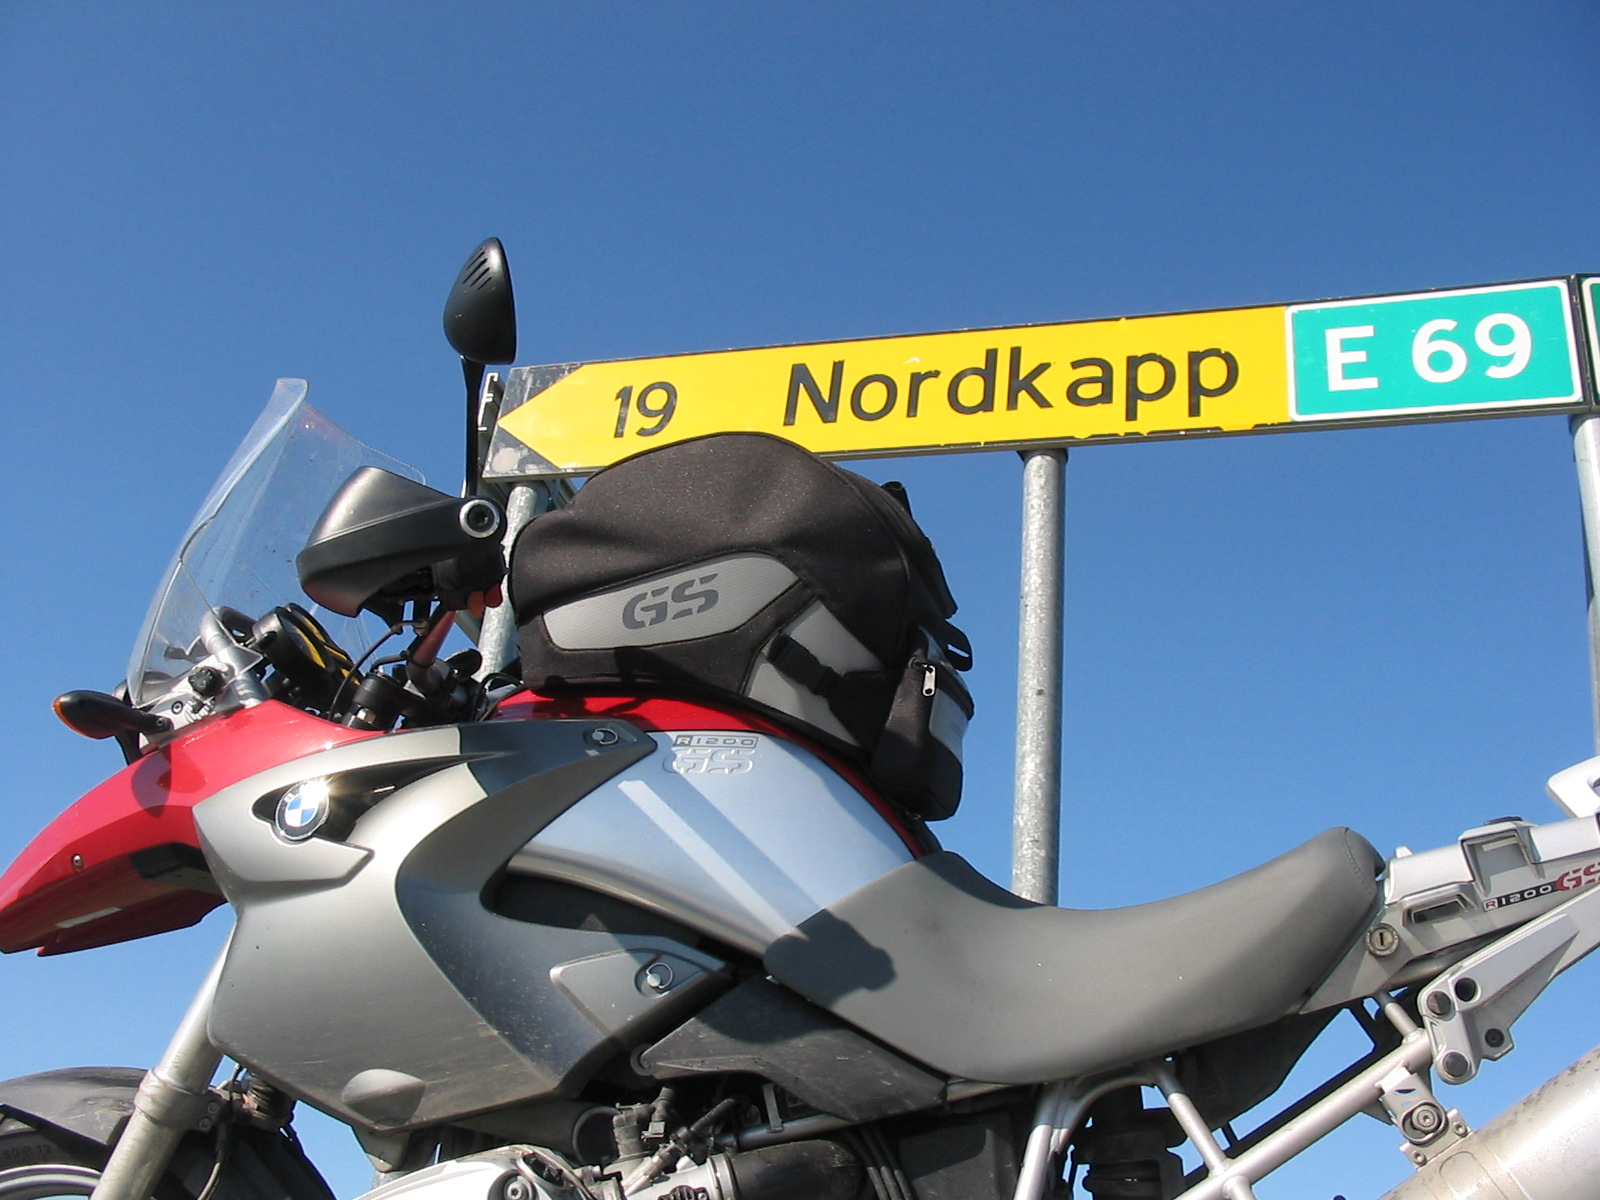
\includegraphics[scale=0.60]{images/Norwegen_04_116.jpg}
	\caption{Norwegen - Wegweiser}
	\label{fig:Norwegen_04_002}
\end{figure}

\begin{figure}[H]
	\centering
		
\includegraphics{images/HTLstp-RGB.png}
	\caption{Neues HTL - Logo}
	\label{fig:edvo-logo}
\end{figure}

\pagebreak
		
\subsection{Richtiges zitieren}
Dies ist ein w�rtliches Zitat:
\begin{quote}
\textit{Textverarbeitung durch einen Rechner mit dem Ergebnis des Ausdrucks in Buchqualit�t ist durch die Entwicklung geeigneter Programme in den letzten Jahren m�glich geworden.}\cite[Seite 3]{kopka1:00}
\end{quote}
Bezug auf eine bestimmte Quelle in einem Buch:\\
Dieser Sachverhalt wird in \cite[Seite 17ff]{demig:04} genauer beschrieben.\\

Eine gute Einf�hrung zu \LaTeX findet man unter \cite{Web:01}

\subsection{Einbinden von PDF - Seiten}

Hier wird (auf der n�chsten Seite) eine externes PDF-Dokument eingef�gt:

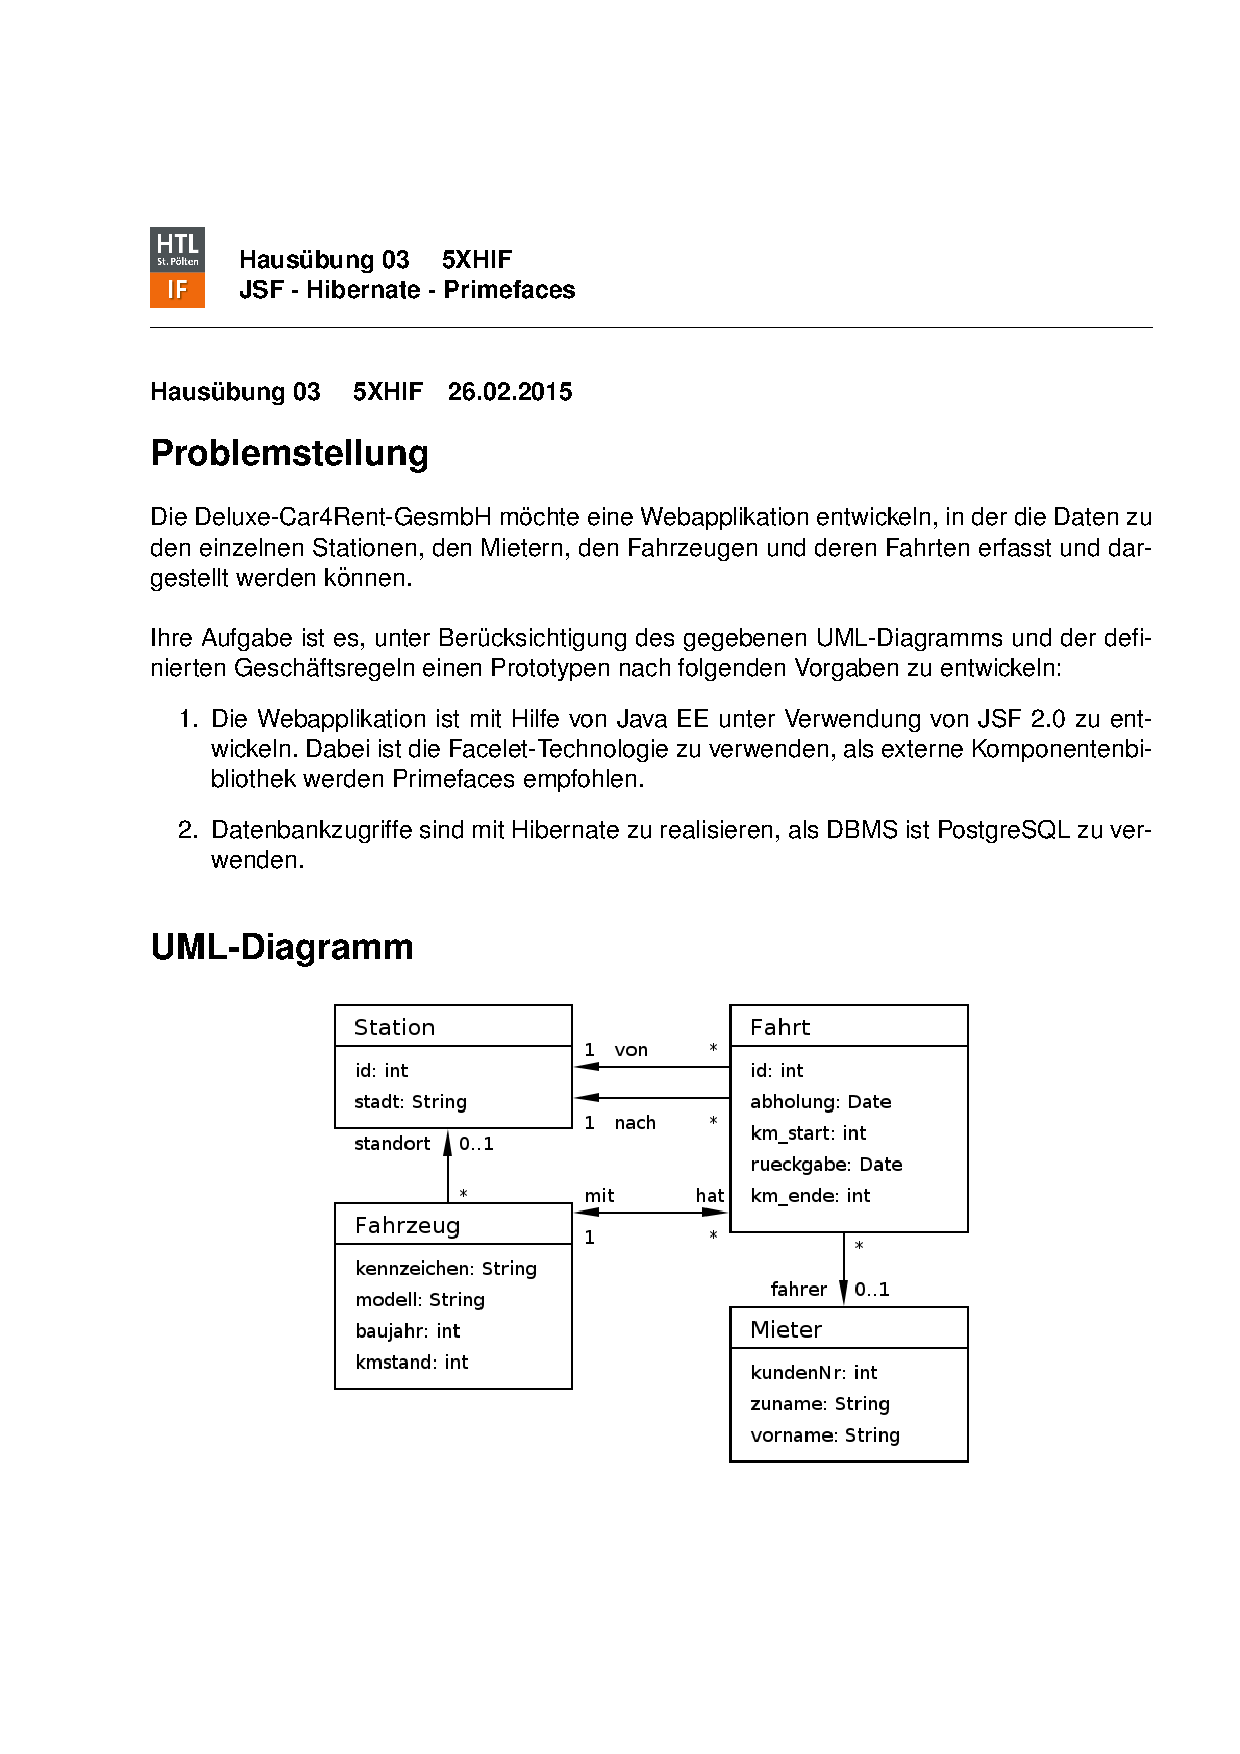
\includepdf[pages={1,2}]{pdf/Hausuebung_03.pdf}



			

		
%\clearpage
	
%--------------------------------------------------------------------------
% Anhang
%--------------------------------------------------------------------------
\begin{comment}


  \phantomsection
  \addcontentsline{toc}{chapter}{Anhang}
	\addcontentsline{toc1}{section}{Abbildungsverzeichnis}
	\listoffigures
	\newpage
	\phantomsection
	
	\addcontentsline{toc}{section}{Tabellenverzeichnis}
	\listoftables
	\newpage
	\phantomsection

	\addcontentsline{toc}{section}{Verzeichnis der Listings}
	\lstlistoflistings
	\newpage
	\phantomsection
	
	%\addcontentsline{toc}{section}{Index}
  \printindex
  \newpage
  \phantomsection
  \end{comment}
	\addcontentsline{toc}{section}{Literaturverzeichnis}
	%\bibliographystyle{alpha} 		 %Standardstyle
	%\bibliographystyle{dinat}		 %Style und Layout nach DIN 1502
	%\bibliography{tiger}					 %Literaturverzeichnis einf�gen
	
	
	%So kann zitiert werden (sollte in einer der Unterdateien sein)
	%\citep[vgl. Seite 22]{kopka1:00}
	\begin{thebibliography}{999}
		\bibitem[Architectural Styles and
		the Design of Network-based Software Architectures]{Web:01}
		\href{https://www.ics.uci.edu/~fielding/pubs/dissertation/fielding_dissertation.pdf}{https://www.ics.uci.edu/~fielding/pubs/dissertation/fielding\_dissertation.pdf}\\
		REST - Definierende Dissertation\\
		19.11.2018
		\bibitem[Architectural Styles and
			the Design of Network-based Software Architectures]{Web:02}
		\href{https://www.ics.uci.edu/~fielding/pubs/dissertation/fielding_dissertation.pdf}{https://www.ics.uci.edu/~fielding/pubs/dissertation/fielding\_dissertation.pdf}\\
		Zitat-Dr. Fielding optionale Funktionalit�t S.84\\
		19.11.2018
		
		
	\end{thebibliography} 
	\newpage
	\phantomsection
\end{document}